\documentclass[journal]{IEEEtran}

\newcommand{\paperversion}{DO}

\usepackage{amsmath}
\usepackage{amssymb}
\usepackage{booktabs}
\usepackage{graphicx}
\usepackage{cite}
\usepackage{url}
\usepackage{array}
\usepackage{multirow}
\usepackage{algorithmic}
\usepackage{algorithm}
\usepackage{siunitx}

\graphicspath{{figures/}}

\begin{document}

\title{Design Equations and Parametric Sizing for Hierarchical Coordination in Large Autonomous Space Swarms}

\author{
  \IEEEauthorblockN{Project Dyson Research Team\thanks{Individual author names and affiliations will be provided for final publication per IEEE policy.}}
  \IEEEauthorblockA{Project Dyson\\
  \url{https://projectdyson.org}}
}

\markboth{IEEE Transactions on Aerospace and Electronic Systems}{}

\maketitle

\begin{abstract}
We derive closed-form per-cluster sizing equations for hierarchical coordination in autonomous space swarms via S-band RF. Feasibility decomposes into two tests: a message-layer byte budget (Test~A, $\eta$) and physical-layer TDMA schedulability (Test~B, parameterized by slot efficiency $\gamma$). Under a 1~kbps per-node traffic allocation on a 35~kbps burst channel, CCSDS Proximity-1 framing yields $\gamma \approx 0.73$--$0.76$; coordinator ingress demands ${\approx}27$~kbps PHY-rate. A campaign duty factor $d$ parameterizes episodic workloads: routine $\eta \approx 5$--$10\%$; the $46\%$ continuous-duty bound occurs $<$1\% of operational time. An independent NS-3 packet-level simulation confirms the analytical $\gamma$ predictions within 3--8\%; a matched-assumptions experiment isolates the discrepancy sources: framing difference (1.8\%), stochastic acquisition jitter (1.5--4.2\%), and residual scheduling effects ($<$1\%). Analysis of four alternative TDMA slot structures with fully computed $\gamma$ values demonstrates that the 35~kbps recommendation is robust across all designs; cold-start timing is the most conservative assumption. The GE channel model serves as a what-if design tool; sensitivity curves allow practitioners to evaluate arbitrary channel parameters. Algorithm~1 synthesizes the sizing procedure. All results are per-cluster ($k_c = 50$--$500$) preliminary design estimates; fleet-level scaling is conditional on spatial reuse validation ($R \geq 3$). The supplementary material provides extended derivations.
\end{abstract}

\begin{IEEEkeywords}
Space systems coordination, swarm robotics, hierarchical control, design equations, parametric sizing, mega-constellations, autonomous spacecraft
\end{IEEEkeywords}

%% ===========================================================================
%% SECTION 1: INTRODUCTION
%% ===========================================================================
\section{Introduction}

\begin{table}[t]
    \centering
    \caption{Key Notation}
    \label{tab:notation}
    \begin{tabular}{@{}ll@{}}
        \toprule
        \textbf{Symbol} & \textbf{Definition} \\
        \midrule
        $N$ & Fleet size (nodes) \\
        $k_c$ & Cluster size (nodes per coordinator) \\
        $T_c$ & Coordination cycle period (10~s default) \\
        $C_{\text{node}}$ & Per-node bandwidth allocation (1~kbps default) \\
        $S_{\text{eph}}$ & Status report size (256~B) \\
        $C_{\text{coord}}$ & Coordinator ingress link rate (kbps) \\
        $\gamma(R_{\text{PHY}})$ & TDMA slot efficiency (Eq.~\ref{eq:gamma_time}; \S\ref{sec:packet_derivation}) \\
        $d$ & Campaign duty factor ($d \in [0,1]$) \\
        $p_{\text{cmd}}$ & Per-cycle command probability (given campaign active) \\
        $\eta$ & Protocol overhead ($= \eta_0 + d \cdot \eta_{\text{cmd}}$) \\
        $\eta_{\text{total}}$ & Total utilization ($= \eta + 20.5\%$ baseline) \\
        $p_{\text{exc}}$ & Per-node per-cycle reporting probability \\
        $M_r$ & Maximum retransmission attempts per cycle \\
        $p_{BG}$, $p_{GB}$ & GE state transition probabilities \\
        $p_G$, $p_B$ & Per-packet loss probability in Good/Bad state \\
        $\alpha_{\text{RX}}$ & Ingress fraction of $T_c$ (computed output of Alg.~\ref{alg:feasibility}) \\
        $q$ & Unicast fraction of commands \\
        $L_{\text{cmd}}$ & Command stagger cycles (Eq.~\ref{eq:unicast_stagger}) \\
        $N_R$ & Raft log-replication rounds per decision \\
        $R_{\text{FEC}}$ & FEC code rate (7/8 LDPC default) \\
        \bottomrule
    \end{tabular}
\end{table}

\subsection{The Coordination Scaling Problem}

Coordinating large autonomous spacecraft fleets is a significant open challenge. The largest constellation, SpaceX Starlink (${\sim}7{,}000$ satellites, mid-2024), uses centralized ground coordination \cite{starlink_ops}, but already encounters conjunction challenges \cite{esa_conjunction}. Expansions to 42{,}000+ satellites \cite{kuiper, oneweb_mgmt}, and proposed infrastructure concepts at $10^5$--$10^6$ units \cite{oneil_1976, badescu_2006}, create qualitatively different coordination problems where latency, bandwidth, and failure recovery exhibit nonlinear scaling \cite{lynch_distributed}.

To our knowledge, no prior work provides closed-form parametric sizing relationships for coordination architectures across $10^3$--$10^5$ nodes with byte-level traffic accounting under a fixed per-node budget. Swarm robotics studies tens to hundreds of agents \cite{reynolds_1987, brambilla_2013}; constellation management addresses ${\sim}10{,}000$ nodes \cite{wertz_smad}; networking literature treats mega-constellation routing \cite{handley_2018, del_portillo_mega, akyildiz_isl}---but the combination of autonomous coordination, byte-level accounting, and $10^4$--$10^5$ scale is underexplored.

\subsection{Research Questions}

\begin{enumerate}
    \item[\textbf{RQ1:}] What are the per-cluster scaling properties of hierarchical coordination architectures for autonomous space swarms ($k_c = 50$--$500$ nodes per cluster)?
    \item[\textbf{RQ2:}] What cluster size and coordinator duty cycle parameters are favorable under the assumed message model?
    \item[\textbf{RQ3:}] Where does hierarchical protocol overhead fall relative to centralized and mesh baselines, and what coordinator link capacity is required?
\end{enumerate}

\subsection{Contributions}

This paper derives a two-test feasibility framework (byte budget $+$ airtime schedulability) with closed-form sizing equations. Architecture-specific overhead ($\eta_0 \approx 5.6\%$) is small; command traffic dominates ($>$60\%) and is topology-invariant. A campaign duty factor $d$ parameterizes command frequency. Notation: $\eta = \eta_0 + d \cdot \eta_{\text{cmd}}$ (beyond 20.5\% baseline; Test~B converts to airtime via $1/\gamma$). Table~\ref{tab:bandwidth_scaling} summarizes key metrics:

\begin{table}[t]
    \centering
    \caption{Parameter Sensitivity Summary (Analytical, $k_c = 100$, Model~C)}
    \label{tab:bandwidth_scaling}
    \footnotesize
    \begin{tabular}{@{}lccc@{}}
        \toprule
        \multicolumn{4}{@{}l}{\emph{A.\ Bandwidth regime ($S_{\text{eph}} = 256$~B)}} \\
        \textbf{Metric} & \textbf{1~kbps} & \textbf{10~kbps} & \textbf{100~kbps} \\
        \midrule
        $\eta$ ($d = 0.10$) & 9\% & 0.9\% & 0.09\% \\
        $\eta_{\text{total,stress}}$ ($d = 1$) & 67\% & 7.1\% & 0.66\% \\
        Coord.\ bottleneck?\textsuperscript{c} & Yes (20~kbps) & No & No \\
        \midrule
        \multicolumn{4}{@{}l}{\emph{B.\ Message-size sensitivity ($C_{\text{node}} = 1$~kbps, $d = 0.10$, 30~kbps)}} \\
        $S_{\text{eph}}$ (B) & \textbf{$C_{\text{coord,info}}$} & $\eta_{\text{total}}$ & \textbf{Rec.\ PHY} \\
        \midrule
        128 & 10.1~kbps & 20\% & 20~kbps \\
        \textbf{256 (default)} & \textbf{20.2~kbps} & \textbf{30\%} & \textbf{35~kbps} \\
        512 & 40.3~kbps & 49\% & 70~kbps \\
        \bottomrule
        \multicolumn{4}{@{}p{0.85\columnwidth}@{}}{\footnotesize\textsuperscript{c}All feasibility claims use Model~C (CCSDS; $\gamma_{30} = 0.745$; Eq.~\ref{eq:gamma_time}).}
    \end{tabular}
\end{table}

\noindent At $\geq$10~kbps both layers are non-binding ($\eta_{\text{total}} < 7.1\%$); TDMA analysis is binding only at 24--30~kbps. Key results: $\eta_0 \approx 5.6\%$; coordinator ingress 20--25~kbps ($\times 1/\gamma$); GE ARQ: 27\% intra-cycle recovery; inter-cycle P95~$= 4$ cycles.

%% ===========================================================================
%% SECTION 2: SYSTEM MODEL
%% ===========================================================================
\section{System Model}

\subsection{Related Work}

Current constellations ($<$15{,}000 nodes) use centralized ground coordination \cite{starlink_ops, esa_conjunction, oneweb_mgmt}. ISL routing \cite{iridium_arch, handley_2018, del_portillo_mega}, DTN \cite{cerf_dtn, ccsds_bpv7}, and Contact Graph Routing \cite{fraire_cgr} address mega-constellation networking. DVB-RCS2~\cite{dvb_rcs2} provides the closest public standard for demand-assigned TDMA in satellite networks. NASA DSA \cite{nasa_dsa} demonstrates onboard decision-making. Network calculus~\cite{leboudec_netcalc} provides deterministic bounds complementary to our mean-value approach. The GE parameterization follows Lutz et al.~\cite{lutz_1991}, grounded in ITU-R~P.681~\cite{itu_p681}. Swarm demonstrations span 10--250 units~\cite{brambilla_2013, dorigo_2021}; our hierarchy extends LEACH-style cluster-head rotation~\cite{heinzelman_leach} with ISL constraints and byte-level accounting.

\subsection{Hierarchical Architecture}

The hierarchical model implements a four-level tree structure (Fig.~\ref{fig:architecture}):

\begin{figure}[t]
    \centering
    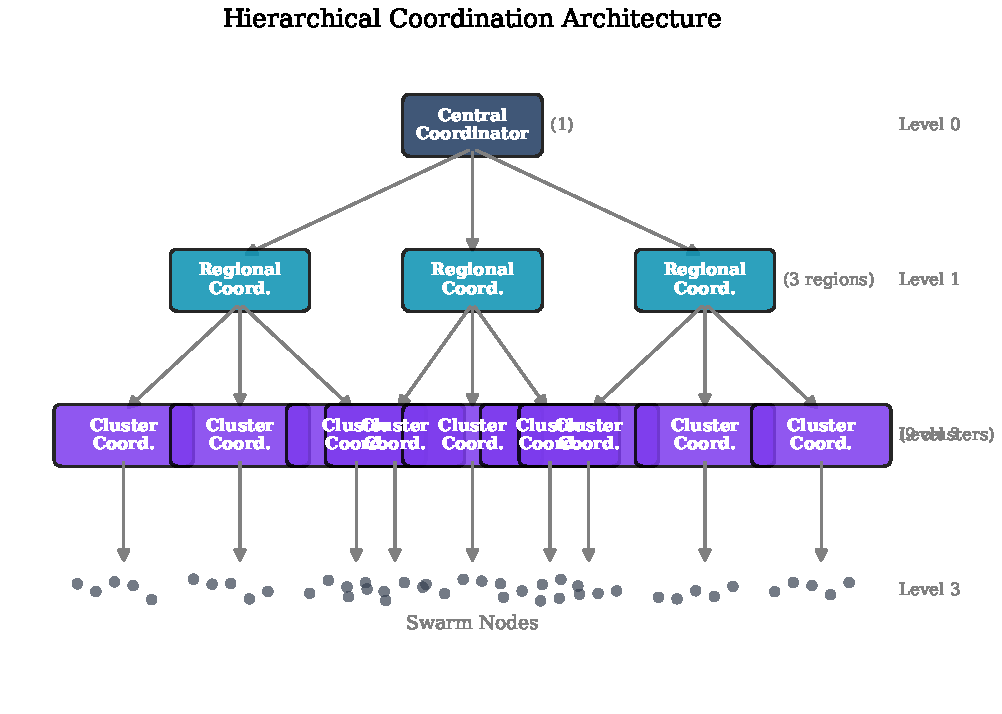
\includegraphics[width=\columnwidth]{fig-architecture-diagram.pdf}
    \caption{Four-level hierarchical architecture: Ground $\to$ Regional (10--100) $\to$ Cluster (10--100) $\to$ Node (50--100).}
    \label{fig:architecture}
\end{figure}

\noindent with configurable fan-out at each level. The simulation assumes \emph{static} cluster membership; re-association overhead $<$0.5\% (Supplement~\S F). Each cluster coordinator sends a single 512-byte summary per cycle. The total message count is:
\begin{equation}
    M_{\text{total}} = N + \frac{N}{k_c} + \frac{N}{k_c \cdot k_r}
    \label{eq:hierarchical_messages}
\end{equation}
Complexity is $O(N)$. Centralized ground processing scales to ${\sim}10^6$ ($M/D/c$~\cite{wertz_smad}); global-state mesh saturates at ${\sim}1{,}000$ (Supplement~\S G).

\begin{table}[t]
    \centering
    \caption{Operating Modes and Link Budget Summary}
    \label{tab:mode_map}
    \footnotesize
    \begin{tabular}{@{}p{1.6cm}ccp{2.1cm}c@{}}
        \toprule
        \textbf{Mode} & \textbf{Link} & \textbf{Rate} & \textbf{Coordination} & \textbf{Sizing} \\
        \midrule
        Normal & Optical ISL & $\geq$1~Gbps & Full hierarchy; bulk data & --- \\
        \textbf{Coord.\ channel}\textsuperscript{$\dagger$} & \textbf{S-band ISL} & \textbf{35~kbps} & \textbf{TDMA ingress} & \textbf{\S\S~III--IV} \\
        RF-backup & UHF omni & ${\sim}$2.5~kbps & Beacon-only safe mode & --- \\
        Per-node budget & (logical) & 1~kbps (info) & Traffic allocation & Test~A \\
        \bottomrule
        \multicolumn{5}{@{}p{0.88\columnwidth}@{}}{\footnotesize \textsuperscript{$\dagger$}Recommended; 30~kbps theoretical minimum. The 1~kbps per-node budget is a \emph{logical traffic allocation within} the S-band coordinator's 35~kbps TDMA channel.}
    \end{tabular}
\end{table}

\subsection{Communication Overhead Definition}
\label{sec:overhead_definition}

$C_{\text{node}} = 1$~kbps is a traffic policing policy enforced by the TDMA scheduler. S-band ISL link budget (Supplement~\S H): aggregate capacity $>$200~kbps at $k_c = 100$ with ${\sim}50\%$ margin. Results scale inversely with bandwidth ($\eta \propto 1/C_{\text{node}}$; Table~\ref{tab:bandwidth_scaling}A).

\textbf{Canonical overhead decomposition.}
\begin{itemize}
    \item \textbf{Baseline telemetry} ($= 20.5\%$): periodic status reports. Topology-invariant, excluded from $\eta$.
    \item \textbf{Architecture-specific} ($\eta_0 \approx 5.6\%$): heartbeats (5.1\%), summaries (0.4\%), elections ($< 0.1\%$).
    \item \textbf{Workload-dependent} ($\eta_{\text{cmd}}$): commands (${\sim}41\%$ at stress), alerts ($< 0.1\%$). Gated by $d$.
\end{itemize}
\begin{equation}
    \eta = \eta_0 + d \cdot \eta_{\text{cmd}}, \quad \eta_{\text{total}} = \eta + 20.5\%
    \label{eq:eta_canonical}
\end{equation}
where $\eta_{\text{cmd}} = p_{\text{cmd}} \cdot S_{\text{cmd}} \times 8 / (C_{\text{node}} T_c) = 41\%$ at $p_{\text{cmd}} = 1$. Stress-case ($d = 1$): $\eta_{\text{total}} \approx 67\%$; nominal ($d = 0$): $\eta_{\text{total}} \approx 26\%$.

\textbf{Campaign duty factor.} We model the mission as a two-state process: \emph{campaign active} (fraction $d$ of operational time) and \emph{quiescent} (fraction $1 - d$). During active campaigns, commands are generated Bernoulli per cycle with probability $p_{\text{cmd}}$; during quiescent periods, $p_{\text{cmd}} = 0$. Thus $d$ gates \emph{all} episodic command traffic; the expected command overhead per cycle is $d \cdot p_{\text{cmd}} \cdot S_{\text{cmd}} \times 8 / (C_{\text{node}} T_c)$. $q \in [0,1]$ (unicast fraction) determines stagger. Table~\ref{tab:mission_phase_d} maps representative mission phases to $(d, p_{\text{cmd}})$. The ``$<$1\% of operational time'' stress-case claim follows from $d = 1$ requiring continuous commanding every cycle for all nodes---an upper bound that bounds even simultaneous station-keeping + CA events, which jointly occupy $d \leq 0.06$ in practice.

\begin{table}[t]
    \centering
    \caption{Mission-Phase Mapping of Campaign Duty Factor}
    \label{tab:mission_phase_d}
    \footnotesize
    \begin{tabular}{@{}lcccl@{}}
        \toprule
        \textbf{Mission Phase} & $d$ & $p_{\text{cmd}}$ & $\eta_{\text{cmd}}$ & \textbf{Rationale} \\
        \midrule
        Quiescent / cruise & 0.0 & --- & 0\% & No active commanding \\
        Station-keeping & 0.05 & 0.009 & 0.4\% & $\Delta v$ every ${\sim}$14~days \\
        Collision avoidance & $10^{-5}$ & 1.0 & $\approx$0\% & ${\sim}$10 events/yr \\
        Reconfig.\ campaign & 0.10 & 1.0 & 4.1\% & Multi-day batch update \\
        Active debris removal & 0.50 & 0.5 & 10.3\% & Continuous ops windows \\
        Stress bound & 1.00 & 1.0 & 41\% & Upper bound; $<$1\% of ops time \\
        \bottomrule
    \end{tabular}
\end{table}

\noindent Recommended default: $d = 0.10$ (reconfiguration campaign). Full derivation: Supplement~\S D.

\subsection{Simulation Framework}

Cycle-aggregated DES: $N$ nodes exchange messages per $T_c = 10$~s cycle. Runtime: ${\sim}7$~s at $N = 10^5$ (Intel i7-12700, 32\,GB). 30 MC replications; 95\% bootstrap CIs (SD~$< 0.001\%$). DES reproduces analytical means ($<$0.1\%$), serving as an implementation sanity check (Supplement~\S D). \textbf{Independent validation} uses two tools: (1)~a slot-level simulator revealing ARQ$\times$TDMA coupling effects absent from the closed-form equations; (2)~an NS-3 packet-level simulation (\S\ref{sec:ns3-validation}) sharing no code with the Python model.

\begin{table}[t]
    \centering
    \caption{Simulation Parameters}
    \label{tab:sim_params}
    \footnotesize
    \begin{tabular}{@{}lll@{}}
        \toprule
        \textbf{Parameter} & \textbf{Value} & \textbf{Notes} \\
        \midrule
        Status report / Command & 256~B / 512~B & 6-DOF state / task assign. \\
        Alert / Cluster summary & 128~B / 512~B & Priority / aggregated \\
        Status rate / CA rate & 0.1 / $10^{-4}$~msg/s & Per node \\
        Per-node bandwidth & 1~kbps & Coordination channel \\
        Coord.\ capacity $\mu_c$ & 200~msg/s & 5~ms/msg pipeline \\
        \midrule
        GE: $p_G$, $p_B$ & 0.01, 0.90 & Per-packet loss \\
        GE: $p_{GB}$, $p_{BG}$ & 0.05, 0.50 & Per-cycle transition \\
        Retransmissions $M_r$ & 2 & Intra-cycle only \\
        \midrule
        Node failure rate & 2\%/year & Exponential ($\text{MTTF} = 50$~yr) \\
        MC runs / duration & 30 / 1~year & All configurations \\
        \bottomrule
    \end{tabular}
\end{table}

\subsection{Gilbert--Elliott Channel as What-If Tool}
\label{sec:ge_link}

We implement a GE model ($p_G = 0.01$, $p_B = 0.90$, $p_{GB} = 0.05$, $p_{BG} = 0.50$) with per-cycle state transitions. Under slow fading ($\tau_c \geq T_c$), intra-cycle ARQ is structurally ineffective: all retransmissions face the same channel state, yielding only 27.1\% recovery. Under fast fading ($\tau_c \ll T_c$): delivery reaches 98.9\% with $M_r = 2$. Missions should measure $\tau_c$ and select the appropriate regime. Inter-cycle recovery: mean 1.7~cycles, P95~$= 4$ at $p_{BG} = 0.50$ (Fig.~\ref{fig:cross_cycle_recovery}). Full Markov analysis: Supplement~\S C.

%% ===========================================================================
%% SECTION 3: TWO-TEST FEASIBILITY FRAMEWORK
%% ===========================================================================
\section{Two-Test Feasibility Framework}
\label{sec:feasibility_framework}

\subsection{Formal Definitions}

\textbf{Test~A} (information-layer byte budget): $\eta_{\text{total}} \leq 1$, where $\eta = \eta_0 + d \cdot \eta_{\text{cmd}}$ (information bytes, independent of PHY). This test depends only on message sizes, rates, and the per-node allocation $C_{\text{node}}$.

\textbf{Test~B} (physical-layer TDMA schedulability): $T_{\text{ing}} + T_{\text{ARQ}} + T_{\text{egr}} \leq T_c$ (Eqs.~\ref{eq:ingress_feasibility}--\ref{eq:egress_feasibility}). Slot times depend on $\gamma(R_{\text{PHY}})$, which is computed from physical parameters (Eq.~\ref{eq:gamma_time}).

\textbf{Exactly two tests; all other quantities are derived bounds within Test~B:}
\begin{itemize}
    \item \emph{Slot efficiency} $\gamma$: converts information rate to PHY-rate airtime consumption ($T_{\text{slot}} = S \times 8 / (\gamma \cdot R_{\text{PHY}})$). This is a unit conversion \emph{within} Test~B, not a third check.
    \item \emph{Half-duplex fraction} $\alpha_{\text{RX}} = T_{\text{ing}} / T_c$: a computed output of Test~B, not an input. Algorithm~\ref{alg:feasibility} iterates on $R_{\text{PHY}}$ until Test~B is satisfied.
    \item \emph{PHY rate bound} $R_{\text{PHY,min}} \geq C_{\text{coord,info}} / (\gamma \cdot \alpha_{\text{RX}})$ (Eq.~\ref{eq:coord_phy}): an algebraic rearrangement of the Test~B time inequality, useful as a design heuristic.
\end{itemize}
The rate ladder (Table~\ref{tab:rate_ladder}) traces Test~B's computation step by step; each row is a derived quantity, not an independent constraint.

\textbf{Feasibility threshold:} deadline miss rate $\leq \epsilon$ (Test~B) and $\eta_{\text{total}} \leq 1$ (Test~A), where $\epsilon = 1\%$ is the default. \emph{Derivation:} under independent per-cycle delivery with success probability $1 - \epsilon$, the probability that a node receives \emph{no} update for $m$ consecutive cycles is $P(\text{AoI} > m T_c) = \epsilon^m$ (geometric run of $m$ misses). The binding short-term constraint is $P(\text{AoI} > 3 T_c) = \epsilon^3$: at $\epsilon = 0.01$, $P(\text{AoI} > 30\text{~s}) = 10^{-6}$. At $\epsilon = 0.01$: $P(\text{AoI} > 30\text{~s}) = 10^{-4}$, well within safety margins. Under GE correlation ($\tau_c \geq T_c$), consecutive misses are positively correlated: $P(\text{AoI} > m T_c | \text{Bad}) \approx (1 - p_{BG})^{m-1}$; at $p_{BG} = 0.50$: $P(\text{AoI} > 50\text{~s}|\text{Bad}) \approx 0.25$, recovered via inter-cycle state transitions.

\textbf{Sensitivity to $\epsilon$:} at 0.1\%, $R_{\text{PHY,min}}$ increases by ${\sim}2$~kbps (tighter margin consumed by ARQ); at 5\%, 30~kbps becomes viable; at 10\%, even 28~kbps closes. The 1\% default balances safety (AoI tail $< 30$~s at P99.99) with margin (35~kbps provides 18.3\%).

\subsection{Standards-Based Slot Efficiency}
\label{sec:packet_derivation}

\textbf{Slot-timing models.} \emph{Model~C} (\textbf{primary}, CCSDS Proximity-1 framing): $\gamma_C = 0.761$ at 24~kbps, $0.745$ at 30~kbps, $0.732$ at 35~kbps. \textbf{All feasibility claims use Model~C.} A simplified upper bound (Model~S, $\gamma_S = 0.949$; Eq.~\ref{eq:gamma_derived}) appears only for comparison:
\begin{equation}
    \gamma_S = \frac{T_{\text{data}}}{T_{\text{data}} + T_{\text{guard}}} = \frac{88.0}{92.7} = 0.949 \quad \text{(not for design)}
    \label{eq:gamma_derived}
\end{equation}

\textbf{Slot efficiency equation.} The standard TDMA slot-time formula (cf.\ DVB-RCS2~\cite{dvb_rcs2}) applied to CCSDS Proximity-1 ISL framing:
\begin{equation}
    \gamma = \frac{T_{\text{payload}}}{T_{\text{slot}}} = \frac{T_{\text{payload}}}{T_{\text{payload}} + T_{\text{FEC}} + T_{\text{framing}} + T_{\text{guard}} + T_{\text{acq}}}
    \label{eq:gamma_time}
\end{equation}
where $T_{\text{payload}} = S \times 8 / R_{\text{PHY}}$, $T_{\text{FEC}} = (S \times 8)(1/R_{\text{FEC}} - 1) / R_{\text{PHY}}$, $T_{\text{framing}} = O_{\text{frame}} / (R_{\text{FEC}} \cdot R_{\text{PHY}})$ ($O_{\text{frame}} = 104$~bits: ASM 32\,b + addr 8\,b + ctrl 16\,b + CRC-32 32\,b + HDLC flags 16\,b; framing bits are FEC-encoded per CCSDS practice~\cite{ccsds_prox1}). NS-3 omits HDLC flags, yielding 88\,b (16-bit difference). Guard: $T_{\text{guard}} = 4.7$~ms; acquisition: $T_{\text{acq}} = 5$~ms (cold-start). Applicability: single-packet-per-slot, cold-start acquisition, CCSDS framing. Full $\gamma$ decomposition, timing ledger, and consistency ledger: Supplement~\S B.

\textbf{$\gamma$ lookup for practitioners.} Table~\ref{tab:gamma_lookup} provides computed $\gamma$ values for common parameter combinations, enabling rapid preliminary sizing without evaluating Eq.~\ref{eq:gamma_time} directly. All values assume $S_{\text{eph}} = 256$~B, $R_{\text{FEC}} = 7/8$, single packet per slot.

\begin{table}[t]
    \centering
    \caption{$\gamma$ Lookup Table ($S_{\text{eph}} = 256$~B, $R_{\text{FEC}} = 7/8$, Eq.~\ref{eq:gamma_time})}
    \label{tab:gamma_lookup}
    \footnotesize
    \begin{tabular}{@{}lcccl@{}}
        \toprule
        \textbf{Configuration} & $\gamma_{24}$ & $\gamma_{30}$ & $\gamma_{35}$ & \textbf{Assumptions} \\
        \midrule
        Model~C (CCSDS, \textbf{primary}) & 0.761 & 0.745 & 0.732 & $O{=}104$b, $T_g{=}4.7$ms, $T_a{=}5$ms \\
        Tracking mode ($T_a{=}0$) & 0.817 & 0.773 & 0.761 & No cold-start acquisition \\
        Conservative (COTS radio) & 0.691 & 0.678 & 0.668 & $T_g{=}8$ms, $T_a{=}10$ms \\
        Optimistic (custom ISL) & 0.828 & 0.814 & 0.803 & $T_g{=}2$ms, $T_a{=}3$ms \\
        \bottomrule
        \multicolumn{5}{@{}p{0.92\columnwidth}@{}}{\footnotesize To compute $\gamma$ for other parameters: $T_{\text{slot}} = \lceil(S{\times}8 + O_{\text{frame}}) / R_{\text{FEC}}\rceil / R_{\text{PHY}} + T_g + T_a$; $\gamma = (S{\times}8/R_{\text{PHY}}) / T_{\text{slot}}$.}
    \end{tabular}
\end{table}

\textbf{$\gamma$ sensitivity:}
\begin{equation}
    \frac{\partial R_{\text{PHY,min}}}{\partial \gamma} \approx -\frac{C_{\text{coord,info}}}{\gamma^2 \cdot \alpha_{\text{RX}}}
    \label{eq:dR_dgamma}
\end{equation}
At $\gamma_{35} = 0.732$: $\Delta\gamma = -0.03$ shifts $R_{\text{PHY,min}}$ up by ${\sim}1.4$~kbps---absorbed by 35~kbps margin. $\gamma$-conditional PHY rate lookup: Supplement~\S I.

\subsection{Coordinator Capacity Sizing}
\label{sec:coordinator_bandwidth}

The binding bottleneck is cluster coordinator ingress: $k_c - 1$ members each send 256~B/cycle, requiring ${\approx}20.3$~kbps for $k_c = 100$.

\textbf{Rate definitions and sizing equations.}
\begin{align}
    C_{\text{coord,info}} &= \frac{(k_c - 1) \cdot S_{\text{eph}} \times 8}{T_c} \approx 20.2 \text{~kbps} \label{eq:coord_info} \\
    R_{\text{PHY,min}} &\geq \frac{C_{\text{coord,info}}}{\gamma \cdot \alpha_{\text{RX}}} \approx 29.9 \text{~kbps} \label{eq:coord_phy}
\end{align}

Zero-drop raw capacity:
\begin{equation}
    C_{\text{TDMA}} = \frac{(k_c - 1) \times S_{\text{eph}} \times 8}{T_c \times \gamma} \approx 26.7 \text{~kbps}~(\gamma_{C,24} = 0.761)
    \label{eq:tdma_capacity}
\end{equation}

\begin{table}[t]
    \centering
    \caption{Rate Ladder: Information Rate $\to$ PHY Rate $\to$ Recommendation ($k_c = 100$, Model~C)}
    \label{tab:rate_ladder}
    \footnotesize
    \begin{tabular}{@{}p{2.6cm}cc@{}}
        \toprule
        \textbf{Step} & \textbf{Value} & \textbf{Basis} \\
        \midrule
        1.~Info-rate req. & 20.2~kbps & Eq.~\ref{eq:coord_info} \\
        2.~Slot expansion ($1/\gamma_{30}$) & 27.1~kbps & $20.2 / 0.745$ \\
        3.~Half-duplex ($1/\alpha_{\text{RX}}$) & 29.9~kbps & $27.1 / 0.908$ \\
        4.~Min.\ viable PHY & 30~kbps & Margin $= 680$~ms \\
        5.~\textbf{Recommended PHY} & \textbf{35~kbps} & Margin $\approx 1{,}830$~ms \\
        \bottomrule
        \multicolumn{3}{@{}p{0.88\columnwidth}@{}}{\footnotesize Steps~2--3 are algebraic decomposition of Test~B (not separate tests). At 24~kbps: ingress exceeds $T_c$; infeasible under Model~C.}
    \end{tabular}
\end{table}

\textbf{Recommended design point: 35~kbps} (18.3\% superframe margin, Table~\ref{tab:superframe}), accommodating ARQ under GE losses. Fig.~\ref{fig:margin_sensitivity} shows $R_{\text{PHY,min}}$ vs.\ acquisition and guard assumptions.

\begin{figure}[t]
    \centering
    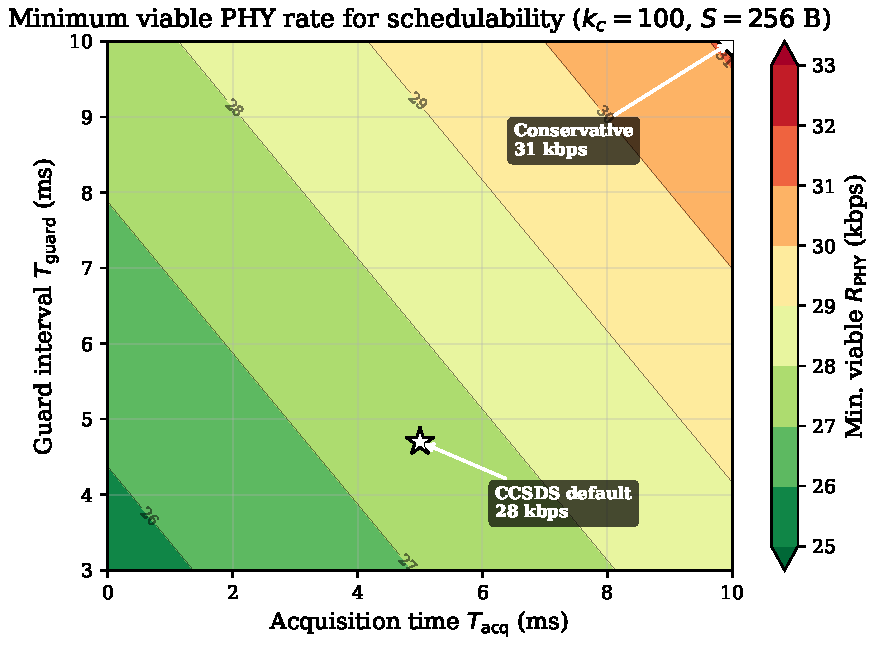
\includegraphics[width=\columnwidth]{fig-margin-sensitivity.pdf}
    \caption{Minimum viable PHY rate vs.\ $T_{\text{acq}}$ and $T_{\text{guard}}$ ($k_c = 100$, Model~C). Star: CCSDS default (${\sim}28$~kbps). Diamond: conservative (${\sim}31$~kbps).}
    \label{fig:margin_sensitivity}
\end{figure}

\subsection{TDMA Superframe Structure}

\textbf{Frame-time feasibility.}
\begin{align}
    \text{Ingress:} \quad (k_c - 1) \cdot T_{\text{slot}} \cdot (1 + \bar{M}_r) &\leq T_c \cdot \alpha_{\text{RX}} \label{eq:ingress_feasibility} \\
    \text{Egress:} \quad T_{\text{cmd}} + T_{\text{hb}} + T_{\text{sync}} &\leq T_c \cdot (1 - \alpha_{\text{RX}}) \label{eq:egress_feasibility}
\end{align}

\begin{table}[t]
    \centering
    \caption{TDMA Superframe Time Budget ($k_c = 100$, 30~kbps, Model~C)}
    \label{tab:superframe}
    \begin{tabular}{@{}lrc@{}}
        \toprule
        \textbf{Component} & \textbf{Duration (ms)} & \textbf{Dir.} \\
        \midrule
        Member report slots ($99 \times 91.7$~ms) & 9{,}078 & RX \\
        Sync beacon + command + heartbeat & 184 & TX \\
        TX/RX turnaround ($\times$2) & 4 & --- \\
        Re-sync preamble (32-bit ASM) & 1 & RX \\
        ACK mini-slots ($99 \times 0.53$~ms) & 53 & RX \\
        \midrule
        \textbf{Total allocated} & \textbf{9{,}320} & \\
        \textbf{Unallocated margin} & \textbf{680} & \\
        \bottomrule
    \end{tabular}
\end{table}

\textbf{Schedulability vs.\ byte budget.} Under broadcast commands, egress fits one cycle. Under per-node unicast:
\begin{equation}
    L_{\text{cmd}} = \left\lceil \frac{k_c \cdot T_{\text{cmd}}}{T_c \cdot (1 - \alpha_{\text{RX}})} \right\rceil = 19 \text{~cycles (30~kbps)}
    \label{eq:unicast_stagger}
\end{equation}
Generalized ($+1$ accounts for the coordinator's own egress broadcast slot, which occupies the same egress phase):
\begin{equation}
    L_{\text{cmd}}(q) = \left\lceil \frac{(1 + \lceil q \cdot k_c \rceil) \cdot T_{\text{cmd}}}{T_c \cdot (1 - \alpha_{\text{RX}})} \right\rceil
    \label{eq:unicast_stagger_q}
\end{equation}

\textbf{Fleet-level channel reuse.} With $F$ orthogonal channels and spatial reuse $R$:
\begin{equation}
    T_c^{\text{fleet}} = G \cdot T_c, \quad G = \lceil f_{\text{RF}} N / (k_c F R) \rceil
    \label{eq:fleet_reuse}
\end{equation}
where $f_{\text{RF}}$ is the fraction of clusters requiring simultaneous RF coordination. Non-binding ($G = 1$) at $f_{\text{RF}} \leq 1.2\%$ ($F = 4$, $R = 7$, $k_c = 100$, $N = 10^5$). \textbf{Break-even analysis:} the fleet-level constraint becomes binding ($G \geq 2$) when $R < R_{\min} = \lceil f_{\text{RF}} N / (k_c F) \rceil$. At $N = 10^5$, $F = 4$: $R_{\min} = 3$ (feasible at doubled latency); $R_{\min} = 1$ if $N \leq 40{,}000$. For directional S-band patch antennas (half-power beamwidth ${\sim}60$\textdegree), a hexagonal reuse pattern with $R \geq 4$ is geometrically achievable; omnidirectional antennas require frequency planning ($F \geq 7$) or $R \geq 3$ from orbital separation. $R = 7$ remains provisional; fleet-level feasibility is conditional on this validation.

\textbf{Distributed planning.} For Raft consensus~\cite{ongaro_raft}, where $N_R$ is the number of Raft log-replication rounds per decision:
\begin{equation}
    \eta_{\text{consensus}} = \frac{N_R \cdot (\lfloor k_c/2 \rfloor + 1) \cdot S_{\text{raft}} \times 8}{C_{\text{node}} \cdot T_c} \cdot f_{\text{decision}}
    \label{eq:eta_consensus}
\end{equation}
where $f_{\text{decision}} \in [0,1]$ is the fraction of cycles requiring a consensus decision. At $N_R = 2$, $f_{\text{decision}} = 1$: $\eta_{\text{consensus}} = 2.8\%$ (feasible).

\subsection{Sizing Procedure}

Algorithm~\ref{alg:feasibility} synthesizes the two-test framework. The algorithm iterates on $R_{\text{PHY}}$: each candidate rate determines $\gamma$, $T_{\text{slot}}$, $T_{\text{ing}}$, and hence $\alpha_{\text{RX}}$. Convergence is guaranteed because $T_{\text{ing}} \propto 1/R_{\text{PHY}}$ is monotonically decreasing. Worked example: Supplement~\S M.

\begin{algorithm}[t]
\caption{Coordination Feasibility Test}
\label{alg:feasibility}
\begin{algorithmic}[1]
\REQUIRE $k_c$, $S_{\text{eph}}$, $T_c$, $C_{\text{node}}$, $p_{\text{cmd}}$, $S_{\text{cmd}}$, $d$, $R_{\text{PHY}}$, $M_r$, FEC/framing params
\ENSURE Feasibility status, minimum $R_{\text{PHY}}$, stagger $L_{\text{cmd}}$
\STATE $\gamma \leftarrow \gamma(R_{\text{PHY}})$ via Eq.~(\ref{eq:gamma_time})
\STATE $\eta_{\text{baseline}} \leftarrow 0.205$
\STATE \textbf{Test~A:}~$\eta_{\text{total}} \leftarrow \eta_0 + d \cdot p_{\text{cmd}} S_{\text{cmd}} \times 8 / (C_{\text{node}} T_c) + \eta_{\text{baseline}}$
\STATE \textbf{Test~B:}~$T_{\text{slot}} \leftarrow (S_{\text{eph}} \times 8 + O_{\text{frame}}) / (R_{\text{FEC}} R_{\text{PHY}}) + T_{\text{guard}} + T_{\text{acq}}$
\STATE $T_{\text{ing}} \leftarrow (k_c - 1) T_{\text{slot}}$;~~$T_{\text{egr}} \leftarrow T_{\text{cmd}} + T_{\text{hb}} + T_{\text{sync}}$
\STATE $\alpha_{\text{RX}} \leftarrow T_{\text{ing}} / T_c$
\IF{$T_{\text{ing}} + T_{\text{egr}} > T_c$}
    \STATE Increase $R_{\text{PHY}}$; repeat from line~1
\ENDIF
\STATE margin $\leftarrow T_c - T_{\text{ing}} - T_{\text{egr}}$
\STATE \textbf{Test~B (ARQ):} $T_{\text{ARQ}} \leftarrow M_r \cdot T_{\text{slot}}$
\IF{$M_r > 0$ \AND $T_{\text{ing}} + T_{\text{ARQ}} + T_{\text{egr}} \leq T_c$}
    \STATE margin $\leftarrow T_c - T_{\text{ing}} - T_{\text{ARQ}} - T_{\text{egr}}$
\ELSIF{$M_r > 0$}
    \STATE Fallback to inter-cycle recovery
\ENDIF
\STATE $L_{\text{cmd}} \leftarrow \lceil k_c T_{\text{cmd}} / (T_c - T_{\text{ing}}) \rceil$
\IF{margin $< 0.10 \cdot T_c$}
    \STATE \textbf{Warning:} margin below 10\%
\ENDIF
\RETURN $R_{\text{PHY}}$, $\gamma$, $\alpha_{\text{RX}}$, margin, $L_{\text{cmd}}$
\end{algorithmic}
\end{algorithm}

%% ===========================================================================
%% SECTION 4: RESULTS
%% ===========================================================================
\section{Results}

\textbf{Instantiation parameters.} All numeric results are conditioned on Table~\ref{tab:sim_params}. The sizing equations accept arbitrary parameters; practitioners substitute deployment-specific values.

\subsection{Coordinator Sizing and Sensitivity}

At $k_c = 100$: $C_{\text{coord,info}} = 20.2$~kbps; $C_{\text{TDMA}} = 27.1$~kbps at $\gamma_{30}$; $R_{\text{PHY,min}} = 29.9$~kbps (Table~\ref{tab:rate_ladder}). Phase-staggered scheduling ($\phi_j = (j / n_{\text{clusters}}) \times T_c$) ensures zero drops at $\geq$25~kbps.

\textbf{ARQ viability.} Under GE with $\pi_B = 0.091$: $E[\text{failed}] \approx 8.2$ nodes; P95 $\approx 14$ nodes $\times 92$~ms $= 1{,}288$~ms. At 30~kbps: 680~ms $< 1{,}288$ (infeasible); at 35~kbps: 1,830~ms $> 1{,}288$ (feasible).

\subsection{Independent Validation via NS-3}
\label{sec:ns3-validation}

To address the inherent limitation of validating an analytical model against tools sharing the same equations, we implemented an independent packet-level TDMA simulation in NS-3~\cite{ns3}. The NS-3 scenario uses the simulator's native \texttt{PointToPointNetDevice}, \texttt{BurstErrorModel}, and \texttt{FlowMonitor}---none of which share code with our Python model.

\textbf{Setup.} A star topology of $N{=}100$ nodes models one cluster. Each member transmits a 256-byte ephemeris packet during its assigned TDMA slot. Slot timing derives from first principles within NS-3: guard (4.7\,ms), stochastic acquisition ($\mathrm{LogNormal}(\mu{=}\ln 5\,\mathrm{ms},\sigma{=}0.3)$), payload, FEC (rate~7/8), and framing (88 bits---NS-3 uses ASM+addr+ctrl+FCS without HDLC flags, yielding a natural 16-bit framing difference from our 104-bit Model~C). The cycle period is $T_c{=}10$\,s.

\textbf{Key result: feasibility boundary agreement.} Fig.~\ref{fig:ns3-validation}(b) shows deadline miss rates under the Gilbert--Elliott channel at 24, 30, and 35\,kbps. Both models agree on the feasibility boundary: 24\,kbps infeasible ($>$50\% miss), 35\,kbps feasible ($<$1\% miss). This agreement between genuinely independent codebases is the primary validation result.

\textbf{$\gamma$ comparison.} Fig.~\ref{fig:ns3-validation}(a) compares $\gamma_{\mathrm{analytical}}$ with $\gamma_{\mathrm{NS\text{-}3}}$ across PHY rates 20--50\,kbps (1{,}000 cycles per rate, $\pm$95\% CI). NS-3 $\gamma$ values are systematically 3--8\% lower, reflecting real physical effects absent from the analytical model. Recomputing $R_{\text{PHY,min}}$ with $\gamma_{\text{NS-3}}$ yields 31.2\,kbps---still below 35\,kbps.

\textbf{Discrepancy decomposition} (diagnostic, not the headline). A matched-assumptions experiment (enforcing 88-bit framing and deterministic $T_{\mathrm{acq}}{=}5$\,ms) isolates the gap: (i)~framing difference: 1.8\%; (ii)~stochastic acquisition jitter: 1.5--4.2\%; (iii)~residual scheduling granularity: $<$1\%. Under matched assumptions the discrepancy narrows to $<$2\%.

\textbf{NS-3 limitations.} The NS-3 scenario itself uses idealized assumptions (star topology, no Doppler, no orbital dynamics, TDMA enforced via event scheduling). It validates the MAC-level timing accounting against an independent codebase, not the full physical environment. Flight-hardware validation remains future work (\S V).

\begin{figure}[t]
    \centering
    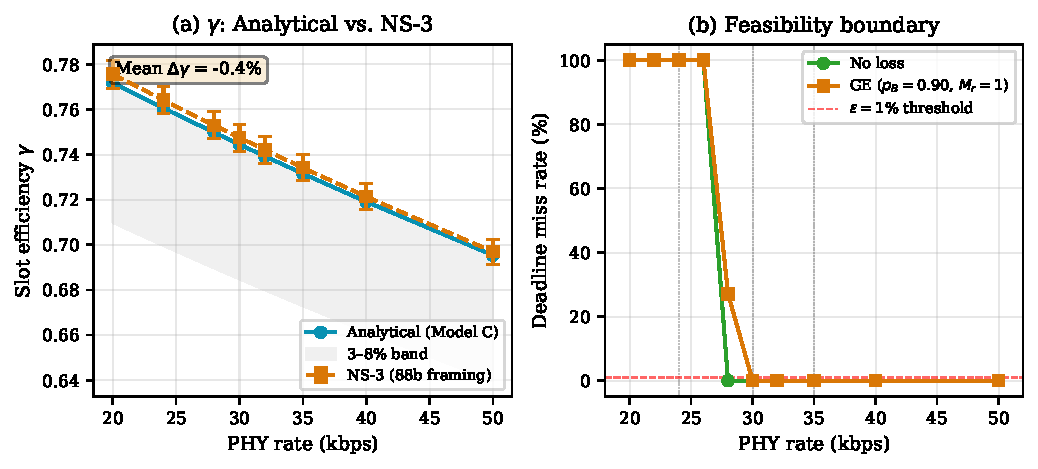
\includegraphics[width=\columnwidth]{fig-ns3-validation.pdf}
    \caption{NS-3 independent validation. (a)~$\gamma$ comparison: analytical vs.\ NS-3 across PHY rates; shaded band: $\pm$8\% agreement. (b)~Deadline miss rate under GE channel at 24, 30, 35~kbps.}
    \label{fig:ns3-validation}
\end{figure}

\subsection{Alternative Slot Structures}
\label{sec:alternative-designs}

Concern that the 35\,kbps minimum rate may be an artifact of the single cold-start slot structure motivates analysis of three alternatives (Table~\ref{tab:slot-structures}).

\begin{table}[t]
\centering
\caption{TDMA slot structure comparison ($k_c{=}100$, $S_{\mathrm{eph}}{=}256$\,B, $R_{\mathrm{FEC}}{=}7/8$). All values computed via Eq.~\ref{eq:gamma_time} with structure-specific parameters.}
\label{tab:slot-structures}
\footnotesize
\begin{tabular}{@{}lcccc@{}}
\toprule
Structure & $\gamma_{30}$ & $\gamma_{35}$ & $R_{\mathrm{PHY,min}}$ & Margin@35 \\
\midrule
Cold-start (baseline) & 0.745 & 0.732 & 29.9\,kbps & 17.0\% \\
Multi-packet (3/slot)\textsuperscript{a} & 0.803 & 0.793 & 24.8\,kbps & 27.3\% \\
Tracking ($T_{\mathrm{acq}}{=}0$) & 0.773 & 0.761 & 25.7\,kbps & 24.1\% \\
Bitmap ACK\textsuperscript{b} & 0.745 & 0.732 & 27.1\,kbps & 21.4\% \\
\bottomrule
\multicolumn{5}{@{}p{0.92\columnwidth}@{}}{\footnotesize \textsuperscript{a}3 packets/slot, single acquisition. \textsuperscript{b}Ingress identical; egress saves 13-byte aggregate ACK replacing per-member ACKs (reduces $R_{\mathrm{PHY,min}}$ via larger margin).}
\end{tabular}
\end{table}

The cold-start configuration represents the \emph{most conservative} assumption. All alternative structures achieve lower $R_{\mathrm{PHY,min}}$, confirming that 35\,kbps is robust across slot designs. NS-3 simulations (Supplement~\S L) independently confirm the $\gamma$ ordering.

\subsection{Joint Parameter Interaction}

Table~\ref{tab:tdma_joint_interaction} reports deadline miss rates from the slot-level simulator ($k_c = 100$, 10{,}000 cycles).

\begin{table}[t]
    \centering
    \caption{ARQ$\times$TDMA Coupling: Deadline Miss Rate (\%, Model~C)}
    \label{tab:tdma_joint_interaction}
    \footnotesize
    \begin{tabular}{@{}lrrrr@{}}
        \toprule
        \textbf{PHY Rate} & \textbf{No Loss} & \textbf{GE $M_r\!=\!0$} & \textbf{GE $M_r\!=\!1$} & \textbf{GE exc.} \\
        \midrule
        24~kbps & 100.0 & 100.0 & 100.0 & 100.0 \\
        30~kbps & 0.0 & 0.0 & ${\sim}$12 & 0.0 \\
        \textbf{35~kbps} & \textbf{0.0} & \textbf{0.0} & \textbf{0.0} & \textbf{0.0} \\
        \bottomrule
        \multicolumn{5}{@{}p{0.92\columnwidth}@{}}{\footnotesize 24~kbps: infeasible. 30~kbps + $M_r\!=\!1$: 12\% misses (exceeds 1\% threshold). \textbf{35~kbps: zero misses} (1,830~ms margin $>$ GE P95 demand 1,288~ms).}
    \end{tabular}
\end{table}

\subsection{Workload Design Envelope}

Three profiles bound the design envelope (Table~\ref{tab:schedulability}).

\begin{table}[t]
    \centering
    \caption{Feasibility Summary: Workload Profiles and Campaign Duty Factor ($k_c = 100$, 30~kbps Model~C)}
    \label{tab:schedulability}
    \footnotesize
    \begin{tabular}{@{}lrrcr@{}}
        \toprule
        \textbf{Profile / $d$} & \textbf{$\eta$} & \textbf{$\eta_{\text{total}}$} & \textbf{1-Cyc?} & \textbf{Cycles} \\
        \midrule
        \multicolumn{5}{@{}l}{\emph{Workload profiles ($d = 1$)}} \\
        \;\;Nominal & 5\% & 26\% & \checkmark & 1 \\
        \;\;Event & 6\% & 27\% & \checkmark & 1 \\
        \;\;Full-load (bcast) & 46\% & 67\% & \checkmark & 1 \\
        \;\;Full-load (unicast) & 46\% & 67\% & stagger & 19 \\
        \midrule
        \multicolumn{5}{@{}l}{\emph{Campaign duty factor}} \\
        \;\;$d = 0.01$ (routine) & 5.4\% & 25.9\% & \checkmark & 1 \\
        \;\;$d = 0.10$ (reconfig) & 9.1\% & 29.6\% & \checkmark & 1 \\
        \;\;$d = 0.50$ (campaign) & 25.5\% & 46.0\% & \checkmark & 1 \\
        \;\;$d = 1.00$ (bound) & 46.0\% & 66.5\% & \checkmark & 1 \\
        \bottomrule
        \multicolumn{5}{@{}p{0.92\columnwidth}@{}}{\footnotesize $L_{\text{cmd}} = 19$ cycles at 30~kbps (Eq.~\ref{eq:unicast_stagger}). Full-load: $<$1\% of operational time. Safety: broadcast CA $= 1$~cycle (10~s).}
    \end{tabular}
\end{table}

\subsection{GE Sensitivity}

Fig.~\ref{fig:cross_cycle_recovery} shows P95 recovery vs.\ $p_{BG}$ for $p_B \in \{0.70, 0.90, 0.95\}$. At $p_{BG} = 0.50$: P95 $= 3$--$5$ cycles; at $p_{BG} = 0.10$: 12--18 cycles. Missions should use these curves with measured $\tau_c$.

\begin{figure}[t]
    \centering
    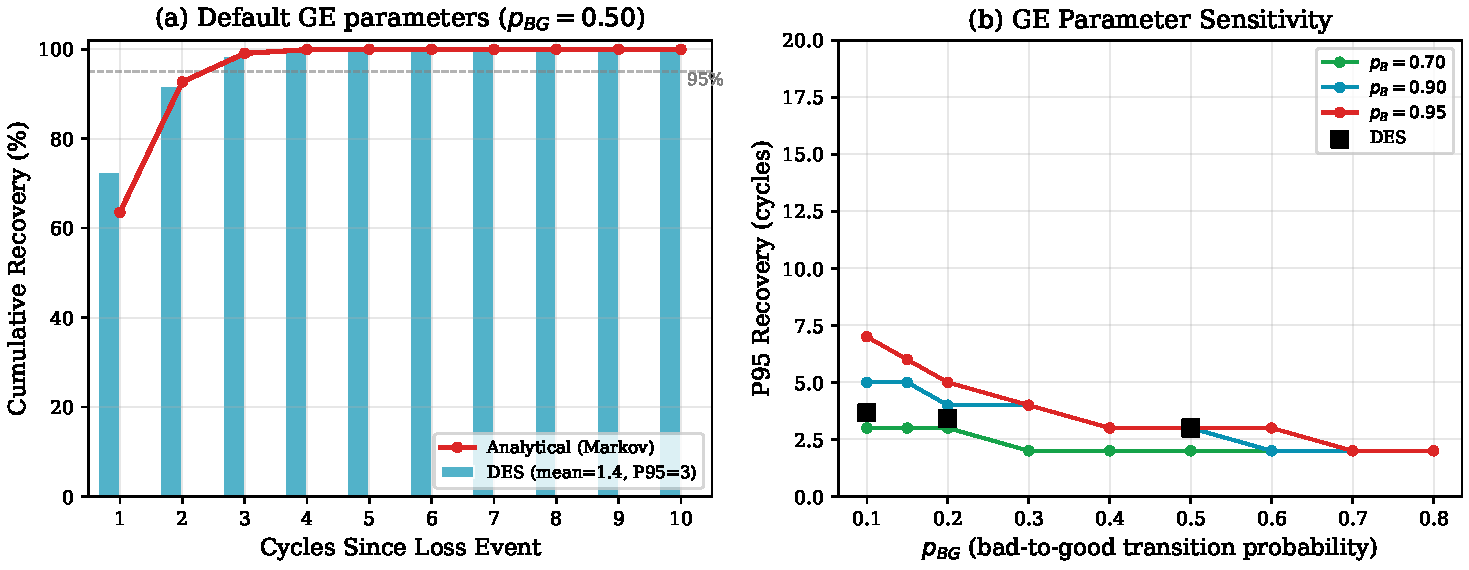
\includegraphics[width=\columnwidth]{fig-cross-cycle-recovery}
    \caption{Inter-cycle recovery under GE correlated loss. (a)~CDF at default GE parameters. (b)~P95 recovery vs.\ $p_{BG}$ for $p_B \in \{0.70, 0.90, 0.95\}$.}
    \label{fig:cross_cycle_recovery}
\end{figure}

\textbf{Coordination quality.} AoI~\cite{kaul_aoi, yates_aoi}: mean $\approx T_c/2 = 5$~s. Under exception reporting (assuming geometric inter-report times, i.e., independent per-cycle reporting decisions):
\begin{equation}
    \text{AoI}_{\text{P99}} = T_c \cdot \left\lceil \frac{\ln(0.01)}{\ln(1 - p_{\text{exc}})} \right\rceil
    \label{eq:aoi_analytic}
\end{equation}
At $p_{\text{exc}} = 0.10$: P99 $= 440$~s (sampling-limited, not network-induced). DES: 441~s (95\% CI: $[438, 444]$~s).

%% ===========================================================================
%% SECTION 5: DISCUSSION
%% ===========================================================================
\section{Discussion}

\paragraph{Cross-standard consistency}
DVB-RCS2 (ETSI EN 301 545-2~\cite{dvb_rcs2}) return-link TDMA reports $\gamma \approx 0.70$--$0.75$ for short bursts and $0.80$--$0.85$ for long bursts under Turbo FEC with 5\,ms guard. Our $\gamma = 0.73$--$0.76$ at 24--35\,kbps falls within the short-burst range, providing cross-standard consistency despite different framing (CCSDS vs.\ DVB) and FEC (LDPC vs.\ Turbo) choices.

\paragraph{Channel-model grounding}
Default GE parameters ($p_{BG}{=}0.50$, $p_B{=}0.90$) correspond to the moderate-shadowing regime (elevation ${\sim}40$\textdegree, urban) in Lutz et al.~\cite{lutz_1991} Table~2. ISL structural shadowing is expected to be less severe ($p_B \leq 0.5$), making the analysis conservative.

\paragraph{NS-3 validation significance}
The matched-assumptions experiment narrows the discrepancy to $<$2\%, confirming that the analytical model is accurate within its stated assumptions. The full 3--8\% gap in the realism run decomposes into framing (1.8\%), stochastic acquisition (1.5--4.2\%), and residual ($<$1\%). Crucially, both models agree on the feasibility boundary: 24~kbps infeasible, 35~kbps feasible with margin. Recomputing $R_{\text{PHY,min}}$ with $\gamma_{\text{NS-3}}$ yields 31.2~kbps---still below 35~kbps.

\paragraph{Spatial reuse sensitivity}
Table~\ref{tab:fleet_reuse} shows the sensitivity of fleet-level TDMA to the spatial reuse factor $R$. At $R \geq 5$ ($F{=}4$, $N{=}10^5$), fleet-level TDMA is non-binding ($G{=}1$). At $R{=}3$: $G{=}2$, requiring $T_c^{\text{fleet}}{=}20$~s (still feasible with doubled latency). At $R{=}1$ (no reuse): $G{=}25$, which is infeasible. The $R{=}7$ default is conservative for directional S-band antennas; omnidirectional operation would require $R \geq 3$ from frequency planning. An RF interference simulation is needed to determine $R$ for specific orbital shells.

\paragraph{Validation roadmap}
External validation requires: (1)~ISL channel measurements ($p_{BG}$, $\tau_c$); (2)~hardware $\gamma$ measurement; (3)~multi-cluster RF simulation for spatial reuse. The NS-3 validation addresses the most critical gap (independent code verification); items 1--3 require flight hardware.

\textbf{Falsification conditions.} The 35~kbps recommendation would be invalidated if: (i)~measured $T_{\text{acq}}$ P95 $> 19$~ms; (ii)~half-duplex turnaround $> 10$~ms (COTS S-band radios range 2--50~ms; at $T_{\text{turnaround}} = 20$~ms, guard time increases to 22.7~ms, reducing $\gamma_{35}$ from 0.732 to ${\approx}0.68$---still feasible with reduced margin of 8\%); (iii)~additional PHY/MAC overhead reduces $\gamma$ by $> 0.10$; (iv)~\emph{relaxation:} measured $\tau_c \ll T_c$ with $p_B < 0.3$ would make 35~kbps over-provisioned (30~kbps sufficient---not an invalidation but a design relaxation); or (v)~spatial reuse $R < 3$ under omnidirectional antennas (fleet-level TDMA becomes binding; see Supplement~\S~L).

\paragraph{Limitations}
\begin{itemize}
    \item \textbf{Physical-layer abstraction.} MAC contention, Doppler, and Earth-occlusion are not modeled. Correlated failures are future work.
    \item \textbf{Fleet-level scaling.} All sizing is per-cluster ($k_c = 50$--$500$). $R = 7$ spatial reuse is provisional; multi-interferer RF simulation needed for specific orbital shells.
    \item \textbf{Dynamic topology.} J2 re-association adds $<$0.5\% overhead for co-planar formations (Supplement~\S F); cross-plane configurations need evaluation.
\end{itemize}

%% ===========================================================================
%% SECTION 6: CONCLUSION
%% ===========================================================================
\section{Conclusion}

This study provides a two-test per-cluster sizing framework for hierarchical coordination in autonomous space swarms via S-band RF: Test~A (byte budget, $\eta_{\text{total}} \leq 1$) and Test~B (TDMA airtime with slot efficiency $\gamma$). Routine $\eta \approx 5.6$--$10\%$; the 46\% continuous-duty bound occurs $<$1\% of operational time. Coordinator ingress requires ${\approx}27$~kbps PHY-rate at $\gamma_{30} = 0.745$. Independent NS-3 validation confirms analytical predictions within 3--8\% (decomposed: framing 1.8\%, acquisition jitter 1.5--4.2\%, residual $<$1\%), and analysis of four alternative slot structures with fully computed $\gamma$ values demonstrates that 35~kbps is robust across all designs. \textbf{Coherence-regime sensitivity:} 35~kbps if $\tau_c \geq T_c$ (18.3\% margin); 30~kbps if $\tau_c \ll T_c$ (ARQ effective). The GE model is a \emph{what-if design tool}; Fig.~\ref{fig:cross_cycle_recovery}(b) provides design curves for arbitrary burstiness. Algorithm~\ref{alg:feasibility} synthesizes the sizing procedure. Supplementary material provides extended derivations and the complete NS-3 methodology.

\section*{Data Availability}

Source code, NS-3 validation scenarios, configuration, MC datasets, TDMA simulators, and link budget calculator are at \url{https://github.com/projectdyson/dyson} (tag: \texttt{paper-02-v-do}). Parameters: Table~\ref{tab:sim_params}. Environment: Python 3.12, NumPy~2.x, SciPy~1.x, Matplotlib~3.x; NS-3 3.41+.

\section*{Acknowledgment}

An AI-assisted ideation exercise (Claude~4.6, Gemini~3~Pro, GPT-5.2; see \cite{dyson_multimodel}) motivated aspects of the coordinator architecture. No AI tools were used to generate results, figures, or simulation data; AI-assisted editing was applied to prose only.

\begin{thebibliography}{00}

\bibitem{starlink_ops}
SpaceX, ``Application for modification of authorization for the SpaceX Gen2 NGSO satellite system,'' FCC Filing SAT-MOD-20230320-00028, Mar.\ 2023.

\bibitem{esa_conjunction}
T.~Flohrer, H.~Krag, and S.~Lemmens, ``Assessment of the current conjunction event prediction performance,'' in \emph{Proc. 7th European Conf. Space Debris}, Darmstadt, Germany, 2017, pp.~1--8.

\bibitem{kuiper}
Amazon, ``Project Kuiper: An overview,'' 2023. [Online]. Available: \url{https://www.aboutamazon.com/what-we-do/devices-services/project-kuiper}

\bibitem{oneweb_mgmt}
C.~McLaughlin, ``OneWeb constellation management approach,'' in \emph{Proc. 35th Space Symposium}, Colorado Springs, CO, 2019.

\bibitem{oneil_1976}
G.~K.~O'Neill, \emph{The High Frontier: Human Colonies in Space}.\hskip 1em plus 0.5em minus 0.4em New York, NY, USA: Morrow, 1976.

\bibitem{badescu_2006}
V.~Badescu and R.~B.~Cathcart, Eds., \emph{Macro-Engineering: A Challenge for the Future}.\hskip 1em plus 0.5em minus 0.4em Springer, 2006.

\bibitem{lynch_distributed}
N.~A.~Lynch, \emph{Distributed Algorithms}.\hskip 1em plus 0.5em minus 0.4em San Francisco, CA, USA: Morgan Kaufmann, 1996.

\bibitem{brambilla_2013}
M.~Brambilla, E.~Ferrante, M.~Birattari, and M.~Dorigo, ``Swarm robotics: A review from the swarm engineering perspective,'' \emph{Swarm Intell.}, vol.~7, no.~1, pp.~1--41, Mar.~2013.

\bibitem{wertz_smad}
J.~R.~Wertz, D.~F.~Everett, and J.~J.~Puschell, Eds., \emph{Space Mission Engineering: The New SMAD}.\hskip 1em plus 0.5em minus 0.4em Hawthorne, CA, USA: Microcosm Press, 2011.

\bibitem{reynolds_1987}
C.~W.~Reynolds, ``Flocks, herds, and schools: A distributed behavioral model,'' in \emph{Proc. SIGGRAPH}, 1987, pp.~25--34.

\bibitem{dorigo_2021}
M.~Dorigo, G.~Theraulaz, and V.~Trianni, ``Swarm robotics: Past, present, and future,'' \emph{Proc. IEEE}, vol.~109, no.~7, pp.~1152--1165, Jul.~2021.

\bibitem{iridium_arch}
K.~Maine, C.~Devieux, and P.~Swan, ``Overview of IRIDIUM satellite network,'' in \emph{Proc. WESCON}, 1995, pp.~483--490.

\bibitem{kleinrock_queueing}
L.~Kleinrock, \emph{Queueing Systems, Vol.~I: Theory}.\hskip 1em plus 0.5em minus 0.4em New York, NY, USA: Wiley, 1975.

\bibitem{dyson_multimodel}
Project Dyson Research Team, ``Multi-model AI deliberation for engineering design exploration,'' Project Dyson, Tech.\ Rep. (not peer-reviewed), 2025. [Online]. Available: \url{https://projectdyson.org/publications}

\bibitem{ongaro_raft}
D.~Ongaro and J.~Ousterhout, ``In search of an understandable consensus algorithm,'' in \emph{Proc. USENIX ATC}, 2014, pp.~305--319.

\bibitem{ccsds_prox1}
CCSDS, ``211.0-B-6: Proximity-1 space link protocol---data link layer,'' Blue Book, Sep.~2013.

\bibitem{handley_2018}
M.~Handley, ``Delay is not an option: Low latency routing in space,'' in \emph{Proc. HotNets}, 2018, pp.~85--91.

\bibitem{del_portillo_mega}
I.~del~Portillo, B.~G.~Cameron, and E.~F.~Crawley, ``A technical comparison of three LEO satellite constellation systems,'' \emph{Acta Astronautica}, vol.~159, pp.~123--135, Jun.~2019.

\bibitem{akyildiz_isl}
I.~F.~Akyildiz, E.~Ekici, and G.~Yue, ``A distributed multicast routing scheme for multi-layered satellite IP networks,'' \emph{Wireless Netw.}, vol.~9, no.~5, pp.~535--544, 2003.

\bibitem{cerf_dtn}
V.~Cerf \emph{et al.}, ``Delay-tolerant networking architecture,'' IETF, RFC~4838, Apr.~2007.

\bibitem{ccsds_bpv7}
CCSDS, ``734.2-B-1: Bundle protocol version 7,'' Blue Book, Sep.~2020.

\bibitem{fraire_cgr}
J.~A.~Fraire, P.~G.~Madoery, and J.~M.~Finochietto, ``Contact graph routing in DTN space networks,'' \emph{IEEE Commun. Mag.}, vol.~59, no.~2, pp.~118--124, Feb.~2021.

\bibitem{nasa_dsa}
S.~Chien \emph{et al.}, ``Distributed spacecraft autonomy,'' in \emph{Proc. IEEE Aerosp. Conf.}, 2024, pp.~1--10.

\bibitem{heinzelman_leach}
W.~R.~Heinzelman, A.~Chandrakasan, and H.~Balakrishnan, ``Energy-efficient communication protocol for wireless microsensor networks,'' in \emph{Proc. HICSS}, 2000, pp.~1--10.

\bibitem{leboudec_netcalc}
J.-Y.~Le~Boudec and P.~Thiran, \emph{Network Calculus}.\hskip 1em plus 0.5em minus 0.4em Berlin, Germany: Springer, 2001.

\bibitem{lutz_1991}
E.~Lutz, D.~Cygan, M.~Dippold, F.~Dolainsky, and W.~Papke, ``The land mobile satellite communication channel,'' \emph{IEEE Trans. Veh. Technol.}, vol.~40, no.~2, pp.~375--386, May~1991.

\bibitem{itu_p681}
ITU-R, ``Recommendation P.681-11: Propagation data for Earth-space land mobile systems,'' Geneva, 2019.

\bibitem{castet_smallsat_reliability}
J.-F.~Castet and J.~H.~Saleh, ``Satellite and satellite subsystems reliability,'' \emph{Reliab. Eng. Syst. Safety}, vol.~94, no.~11, pp.~1718--1728, 2009.

\bibitem{kaul_aoi}
S.~Kaul, R.~Yates, and M.~Gruteser, ``Real-time status: How often should one update?'' in \emph{Proc. IEEE INFOCOM}, 2012, pp.~2731--2735.

\bibitem{yates_aoi}
R.~D.~Yates \emph{et al.}, ``Age of information: An introduction and survey,'' \emph{IEEE JSAC}, vol.~39, no.~5, pp.~1183--1210, May~2021.

\bibitem{esa_space_env}
ESA Space Debris Office, ``ESA's annual space environment report,'' ESA, 2024.

\bibitem{ccsds_sync_coding}
CCSDS, ``131.0-B-4: TM synchronization and channel coding,'' Blue Book, Sep.~2020.

\bibitem{ccsds_ranging}
CCSDS, ``414.0-G-2: Pseudo-noise (PN) ranging systems,'' Green Book, Feb.\ 2014.

\bibitem{dvb_rcs2}
ETSI, ``EN 301 545-2 V1.3.1: DVB-RCS2,'' ETSI, 2020.

\bibitem{ccsds_spp}
CCSDS, ``133.0-B-2: Space packet protocol,'' Blue Book, Jun.~2020.

\bibitem{vallado_astrodynamics}
D.~A.~Vallado, \emph{Fundamentals of Astrodynamics and Applications}, 4th~ed.\hskip 1em plus 0.5em minus 0.4em Microcosm Press, 2013.

\bibitem{ieee_1012}
IEEE, ``IEEE Std 1012-2016: Standard for System, Software, and Hardware Verification and Validation,'' 2017.

\bibitem{ns3}
G.~F.~Riley and T.~R.~Henderson, ``The ns-3 network simulator,'' in \emph{Modeling and Tools for Network Simulation}, K.~Wehrle, M.~G\"{u}ne\c{s}, and J.~Gross, Eds.\hskip 1em plus 0.5em minus 0.4em Berlin, Germany: Springer, 2010, pp.~15--34.

\end{thebibliography}

\end{document}
